\documentclass[11pt,a4paper]{article}

\usepackage[utf8]{inputenc}
\usepackage[T1]{fontenc}
\usepackage[british]{babel}
\usepackage{lmodern}
\usepackage{microtype}
\usepackage[a4paper,margin=2.5cm]{geometry}
\usepackage{amsmath,amssymb,amsthm}
\usepackage{bm}
\usepackage{graphicx}
\usepackage{booktabs}
\usepackage{multirow}
\usepackage[numbers,sort&compress]{natbib}
\usepackage{hyperref}
\hypersetup{colorlinks=true,linkcolor=blue!50!black,citecolor=blue!50!black,urlcolor=blue!50!black}
\usepackage{xcolor}
\usepackage{caption}
\captionsetup{font=small,labelfont=bf,margin=10pt}
\usepackage{authblk}
\usepackage{tikz}
\usetikzlibrary{positioning,arrows.meta,fit}

\renewcommand{\arraystretch}{1.15}

\newcommand{\Lam}{\Lambda}
\newcommand{\mll}{m_{\ell\ell}}
\newcommand{\sigsm}{\sigma_{\rm SM}}
\newcommand{\Ainv}{\bm{A}^{-1}}
\newcommand{\Phib}{\bm{\Phi}}
\newcommand{\psib}{\bm{\psi}}
\newcommand{\Mref}{M_{\rm ref}}

\title{\bfseries A closed-form attention foundation model for amortised SMEFT inference in Drell-Yan}

\author[1]{Vincent Croft}
\affil[1]{\small\itshape Hackathon submission, Arize track, Google Cloud Rapid Agent Hackathon, May 2026}

\date{\today}

\begin{document}
\maketitle

\begin{abstract}
\noindent
We present a foundation model for inference of dimension-six Standard Model Effective Field Theory (SMEFT) effects in neutral-current Drell-Yan, built so that the forward pass never sees a Wilson coefficient. A learned feature map $\psib_\theta$ is meta-trained end-to-end through a closed-form linear-attention head, in the family proposed by Garnelo and Czarnecki~\cite{Garnelo:2023intention}, with the regression to a query kinematic point solved at inference time by a single ridge inversion in the basis $\psib_\theta(m)$. The model has $5\,328$ parameters and reaches held-out median $R^2 = 0.9997$ on $50$ in-distribution and $50$ out-of-distribution scenarios, with fifth-percentile $R^2$ of $0.96$ in-distribution and $0.93$ out-of-distribution. A parameter-matched DeepSets baseline reaches median $R^2$ of $0.62$ and $0.76$ in the two regions; a regressor that violates the constraint and receives the Wilson vector directly on its forward pass reaches median $R^2$ of $0.94$ in both. The model composes into a closed-loop inference system in which physics-aware drift detectors monitor accuracy, calibration and design-matrix conditioning, the Expected Predictive Information Gain selects high-leverage oracle queries inside the drifted region, and a leverage-stratified split-conformal calibrator is refit after every context update. On an engineered out-of-distribution event in the $|c_{\ell q}^{(3)}| \in [0.6, 1.0]$ band of the analytic Drell-Yan calculator, the loop recovers from a root-mean-square error of $293$ to $2.65$ in $500$ oracle calls, with no gradient-descent step at inference. We argue that closed-form in-context attention is a useful primitive for amortised SMEFT inference and complements the contemporary jet-level foundation model literature, which has so far concentrated on classification benchmarks rather than parameter inference.
\end{abstract}

\section{Introduction}
\label{sec:intro}

Machine learning has become a routine ingredient of analyses at the Large Hadron Collider, from jet tagging to event classification to unbinned likelihood inference. The successes of large self-supervised foundation models in vision and language have prompted a parallel programme in particle physics, with masked-particle modelling~\cite{Heinrich:2024mpm}, contrastive jet representations, OmniJet-$\alpha$~\cite{Birk:2024omnijet}, OmniLearn~\cite{Mikuni:2024omnilearn}, OmniLearned~\cite{Mikuni:2025omnilearned}, HEP-JEPA~\cite{Katel:2025hepjepa} and Sophon~\cite{Sophon:2024} now occupying a recognisable cluster of jet-level foundation models. The shared rhetorical move in this literature is to point to the data-efficiency benefit conferred by self-supervised pre-training on large unlabelled corpora, and to argue that the same benefit can be transferred to high-energy physics if a sufficiently general representation is learned upstream of the downstream task.

The downstream tasks targeted by that programme are almost exclusively classification problems, and the metrics by which success is measured are accuracy, area under the receiver-operating-characteristic curve, and background rejection at fixed signal efficiency. Parameter inference, by which we mean the extraction of an underlying continuous theory parameter from the observed event distribution, sits awkwardly in this picture. The machine learning for effective field theory line of work, beginning with the \textit{Mining Gold} prescription of Brehmer, Cranmer, Louppe and Pavez~\cite{Brehmer:2018kdj} and continuing through the MadMiner software~\cite{Brehmer:2019xox} and the parametrised-classifier formulation of Chen, Glioti, Marzocca, Nardini and Wulzer~\cite{Chen:2022lcp}, has shown how the simulator-supplied joint score and joint likelihood ratio enable model-independent extraction of effective field theory coefficients. None of these methods, however, is a foundation model in the in-context learning sense: each fitted regressor or classifier is bespoke to a fixed Wilson configuration sampled at training time, and a new region of the coefficient space requires retraining.

We argue in this paper that the natural object to amortise across the SMEFT parameter space is not the conditional density itself but the inference problem. Given a thin sample of measured events at an unknown set of Wilson coefficients, the inference problem is the regression of an observed kinematic distribution onto the underlying theory parameter, with the simulator playing the role of the prior over distributions. Closed-form linear attention~\cite{Garnelo:2023intention} solves a ridge-regression problem in a learned feature map at inference time, in a single matrix solve, with no gradient-descent step. The feature map can be trained once on simulations drawn from a broad prior over Wilson coefficients; deployment is a context-set forward pass.

A foundation model of this kind admits a hard architectural constraint that we adopt and motivate. The forward pass must not see a Wilson coefficient. Not as a raw value, not as a polynomial feature, not as a conditioning vector. Wilson coefficients live exclusively in the data-generating process inside the simulator and in the construction of the loss. The architectural reason is that the dimension-six SMEFT cross section is a quadratic polynomial in the coefficients, and a regressor that consumes that polynomial as input has the parametric form of the answer written into its feature map. Such a regressor will fit the training $c$-box to numerical precision and will fail catastrophically outside it, because the polynomial structure forecloses the kind of out-of-distribution interpolation that an in-context learner needs. The empirical comparison in Section~\ref{sec:results} makes the case directly.

We present three results. First, on a controlled benchmark of held-out SMEFT scenarios over the four-fermion operators of greatest sensitivity in Drell-Yan, the closed-form attention head with a learned basis reaches median $R^2 = 0.9997$ at $5\,328$ parameters, against $0.62$ for a parameter-matched DeepSets encoder and $0.94$ for a regressor that violates the constraint and gets the Wilson vector for free at test time. Second, the learned basis is visibly not a rediscovery of the canonical polynomial basis in $\log(m / \Mref)$; the meta-learning objective discovers a richer set of localised features that the closed-form ridge can resolve. Third, the foundation model composes into a closed-loop inference system, with physics-aware drift detectors gating an EPIG-driven acquisition step and a leverage-stratified split-conformal calibrator restoring honest coverage after every context update. On an engineered out-of-distribution event the loop recovers from a root-mean-square error of $293$ to $2.65$ in $500$ oracle invocations.

The paper is organised as follows. Section~\ref{sec:theory} fixes the SMEFT cross-section conventions in Drell-Yan and describes the analytic and Monte Carlo oracles that supply training and validation data. Section~\ref{sec:architecture} introduces the constraint-respecting closed-form attention head and the meta-learning objective. Section~\ref{sec:training} describes the training and benchmark setup. Section~\ref{sec:results} reports the held-out comparison and the learned-basis analysis. Section~\ref{sec:loop} reports the closed-loop demonstration, including drift detection, acquisition and conformal recalibration. Section~\ref{sec:discussion} positions the result against the contemporary jet-level foundation model literature and against the machine learning for effective field theory line; Section~\ref{sec:conclusions} closes. Appendix~\ref{app:derivations} collects the closed-form derivations.

\section{SMEFT in Drell-Yan and the oracle}
\label{sec:theory}

The dimension-six SMEFT extension of the Standard Model is written as
\begin{equation}
  \mathcal{L}_{\rm SMEFT} \;=\; \mathcal{L}_{\rm SM} \;+\; \sum_i \frac{c_i}{\Lam^2}\,\mathcal{O}_i \;+\; \mathcal{O}(\Lam^{-4}),
  \label{eq:smeft-lag}
\end{equation}
with $\{\mathcal{O}_i\}$ the operators of the Warsaw basis~\cite{Grzadkowski:2010es} and $\Lam$ the effective field theory scale. For neutral-current Drell-Yan production at high invariant dilepton mass, the leading contributions come from the four-fermion operators $\mathcal{O}_{\ell q}^{(1)}$, $\mathcal{O}_{\ell q}^{(3)}$, $\mathcal{O}_{\ell u}$ and $\mathcal{O}_{\ell d}$, with Wilson coefficients $\{c_{\ell q}^{(1)}, c_{\ell q}^{(3)}, c_{\ell u}, c_{\ell d}\}$ that we collect into a four-vector $\bm{c}$. We follow the conventions of Greljo and Marzocca~\cite{Greljo:2017vvb} throughout.

The differential cross section, integrated over angular variables and binned in the invariant dilepton mass $\mll$, decomposes exactly as
\begin{equation}
  \sigma(\bm{c}, \mll) \;=\; \sigsm(\mll) \;+\; \sum_{i} A_i(\mll)\, c_i \;+\; \sum_{i \leq j} B_{ij}(\mll)\, c_i c_j,
  \label{eq:morphing}
\end{equation}
with the linear coefficients $A_i$ originating from interference of the dimension-six amplitude with the Standard Model amplitude, and the quadratic coefficients $B_{ij}$ originating from the squared dimension-six amplitude. At a fixed scale $\Lam$, equation~(\ref{eq:morphing}) is the morphing ansatz adopted by the global SMEFT fit community and is the workhorse of the parametrised-classifier line of work~\cite{Chen:2022lcp}. The four-fermion contributions grow as $(\mll / \Lam)^4$ in the high-mass tail, so the differential cross section is steeply increasing in $\mll$ above the electroweak scale; the same growth produces the strongest experimental sensitivity at high invariant mass.

We use two oracles for the cross section as a function of $(\bm{c}, \mll)$. The first is an analytic leading-order calculation that implements equation~(\ref{eq:morphing}) over the fourteen dimension-six operators of greatest phenomenological interest, convolved with the CT18NNLO parton distribution functions~\cite{Hou:2019ct18} via LHAPDF~\cite{Buckley:2014lhapdf}. The analytic oracle is fast enough that the meta-training loop can be driven against it in minutes of central-processing-unit time, and it is exact within the leading-order ansatz. The second is a MadGraph5\_aMC@NLO~\cite{Alwall:2014mg5} pipeline, used to cross-validate the analytic oracle on a small sample of Wilson configurations; in the validation tier reported here the analytic and Monte Carlo cross sections agree at the per-cent level for $|\bm{c}| \leq 1$ across $\mll \in [0.3, 2.5]$~TeV, with the disagreement growing with $|\bm{c}|$ as expected from the missing $\Lam^{-4}$ contributions in the analytic ansatz. The full ablation is described in Section~\ref{sec:discussion}.

For the architectural development and benchmarks of Sections~\ref{sec:architecture}--\ref{sec:results} we use the analytic oracle. The full-chain demonstration in Section~\ref{sec:loop} likewise runs against the analytic oracle for completability inside the hackathon timeline; the Monte Carlo tier is wired but not exercised, because the chain shape is unchanged by oracle fidelity and only the cost ladder differs.

\section{A closed-form attention foundation model}
\label{sec:architecture}

\subsection{The architectural constraint}
\label{sec:constraint}

We require that the foundation model's forward pass not consume a Wilson coefficient under any encoding. Wilson coefficients enter the data-generating process inside the oracle, which samples $\sigma(\bm{c}, \mll)$ at chosen Wilson configurations, and they enter the construction of the loss, by selecting the training scenarios. They do not enter the network.

The reason is structural. Equation~(\ref{eq:morphing}) is a closed-form polynomial in $\bm{c}$ at fixed $\mll$. A regressor with input features $\bm{\phi}_c(\bm{c}) = \{1, c_a, c_a c_b\}$ tensored against a kinematic basis $\psib_x(\mll)$ has the exact parametric form of equation~(\ref{eq:morphing}); a closed-form ridge fit recovers the morphing coefficients $\{A_i, B_{ij}\}$ to numerical precision on training data that span the parameter box, and fails catastrophically outside the box because the polynomial extrapolation has no inductive bias from the data. We observe this directly. A regressor of this kind, fit on a Wilson box that excludes one operator from the training distribution, returns per-operator $R^2$ of order $-100$ on the held-out operator. The information that distinguishes a foundation model from a regressor is not the architecture as such; it is whether the model learns a representation of the data manifold or whether it has the answer written into its feature map. We adopt the constraint as the cleanest available test that the model is doing the former.

\subsection{Intention as a closed-form ridge head}

We use the closed-form linear-attention head proposed by Garnelo and Czarnecki~\cite{Garnelo:2023intention}, which we refer to throughout as Intention. Given a context of $K$ observations $(M_{{\rm ctx}, i}, Y_{{\rm ctx}, i})$ at known kinematic points $M_{{\rm ctx}, i}$ and corresponding measured cross-section ratios $Y_{{\rm ctx}, i} \equiv \sigma(\bm{c}, M_{{\rm ctx}, i}) / \sigsm(M_{{\rm ctx}, i})$, and a query point $M_q$, the Intention prediction is
\begin{equation}
  \hat{Y}_q \;=\; \psib_\theta(M_q)\,\bigl(\psib_\theta(\bm{M}_{\rm ctx})^\top \psib_\theta(\bm{M}_{\rm ctx}) + \alpha \bm{I}\bigr)^{-1}\,\psib_\theta(\bm{M}_{\rm ctx})^\top\,\bm{Y}_{\rm ctx},
  \label{eq:intention}
\end{equation}
where $\psib_\theta : \mathbb{R} \to \mathbb{R}^{D}$ is a learned feature map, $\alpha$ is a small ridge regulariser and bold symbols stack the context. Equation~(\ref{eq:intention}) is exactly the closed-form solution of the regularised least-squares problem
\begin{equation}
  \bm{w}^\star \;=\; \arg\min_{\bm{w}} \,\sum_{i=1}^K\bigl(\psib_\theta(M_{{\rm ctx}, i})^\top \bm{w} - Y_{{\rm ctx}, i}\bigr)^2 \;+\; \alpha \|\bm{w}\|_2^2,
  \label{eq:ridge}
\end{equation}
with $\hat{Y}_q = \psib_\theta(M_q)^\top \bm{w}^\star$, that is, the prediction of a Bayesian linear regression in the learned basis $\psib_\theta$ with a Gaussian prior and homoscedastic noise. The Garnelo and Czarnecki paper establishes that Linear Attention~\cite{Garnelo:2023intention} is the $\alpha \to \infty$ limit of equation~(\ref{eq:intention}), so Intention is a strict generalisation of Linear Attention, and that finite $\alpha$ admits exact closed-form sequential updates by the Sherman-Morrison identity~\cite{Sherman:1950}, repeated in Appendix~\ref{app:derivations} for completeness.

The Wilson coefficient $\bm{c}$ does not appear in equation~(\ref{eq:intention}). It is encoded only through the labels $\bm{Y}_{\rm ctx}$, which are observed cross-section ratios produced by the oracle at the unknown configuration $\bm{c}$. The model infers the relevant statistics of $\bm{c}$ at inference time by solving the ridge problem in the basis $\psib_\theta(M_{\rm ctx})$, and the inferred linear combination is what governs the prediction at the query.

\subsection{The learned feature map}

We take $\psib_\theta(m)$ to be a three-layer multilayer perceptron $\mathbb{R} \to \mathbb{R}^{64} \to \mathbb{R}^{64} \to \mathbb{R}^{16}$ with GELU activations, applied to the scaled input $\log(m / \Mref)$ with $\Mref = 0.2$~TeV. The network has $5\,328$ trainable parameters. The output dimension $D = 16$ exceeds the four canonical polynomial features used in the fixed-basis variant of equation~(\ref{eq:intention}) and is small enough that the per-scenario ridge solve in equation~(\ref{eq:intention}) is sub-millisecond on a central-processing-unit. We train $\psib_\theta$ by backpropagation through the matrix inverse in equation~(\ref{eq:intention}), using the differentiable solver \texttt{torch.linalg.solve} as the inner operation.

The training objective is the per-scenario mean-squared error between the Intention prediction at $Q = 32$ query points and the oracle truth,
\begin{equation}
  \mathcal{L}(\theta) \;=\; \frac{1}{N_{\rm batch}\,Q}\,\sum_{s=1}^{N_{\rm batch}}\,\sum_{q=1}^{Q}\,\bigl(\hat{Y}_q^{(s)}(\theta) - Y_q^{(s)}\bigr)^2,
  \label{eq:meta-mse}
\end{equation}
with $\hat{Y}_q^{(s)}$ the Intention prediction in scenario $s$ from a context of size $K = 12$ drawn together with the query block. Equation~(\ref{eq:meta-mse}) is a meta-learning objective in the sense that the training signal is the error after the per-scenario inference, not the error of any single inference step. The architecture must therefore discover a basis in which the closed-form ridge generalises across scenarios, which is the in-context analogue of learning a prior over distributions.

The predictive uncertainty at a query $q$ admits a closed form as well. In the homoscedastic Bayesian linear regression on $\psib_\theta$, the predictive variance is
\begin{equation}
  \mathrm{Var}\bigl[\hat{Y}_q\bigr] \;=\; \sigma_y^2 \,\bigl(1 + \mathrm{lev}(q)\bigr), \quad \mathrm{lev}(q) \;\equiv\; \psib_\theta(M_q)^\top \bm{A}^{-1} \psib_\theta(M_q),
  \label{eq:leverage}
\end{equation}
with $\bm{A} \equiv \psib_\theta(\bm{M}_{\rm ctx})^\top \psib_\theta(\bm{M}_{\rm ctx}) + \alpha \bm{I}$ the design matrix and $\sigma_y^2$ the noise variance, estimated from the residuals on the context. The leverage $\mathrm{lev}(q)$ is the Mahalanobis distance of the query in the inverse-design-matrix metric and is the closed-form realisation of the kernel-ridge to Gaussian-process duality~\cite{Rasmussen:2006gp}. We use it as the design-matrix-side drift signal in Section~\ref{sec:loop}.

\subsection{Baselines}

We compare against three baselines. The first is the fixed-basis Intention variant, with $\psib(m) = \{1, \log(m/\Mref), \ldots, \log^4(m/\Mref)\}$ and no trainable parameters; this is the closed-form ridge in a hand-engineered polynomial basis and the fixed-architecture counterpart to the learned variant. The second is a parameter-matched DeepSets~\cite{Heinrich:2024mpm}-style encoder that processes each context observation $(M_{{\rm ctx}, i}, Y_{{\rm ctx}, i})$ through a per-event multilayer perceptron, mean-pools the resulting embeddings, concatenates the query $M_q$, and decodes through a second multilayer perceptron. Its parameter count is $6\,545$, that is, $1.23\times$ the Intention head. The third is the regressor variant that violates the architectural constraint and consumes the Wilson vector $\bm{c}$ directly on its forward pass at test time, mapping $(\bm{c}, M_q) \to \hat{Y}_q$ through a multilayer perceptron of $5\,041$ parameters trained on the flattened $(\bm{c}, m, y)$ triples of the training scenarios. We refer to it throughout as the cheat regressor. It marks the upper bound a constraint-respecting architecture would be expected to reach.

\section{Training and benchmark}
\label{sec:training}

The held-out benchmark of this section uses a controlled polynomial-toy oracle. The oracle samples $\mu(\bm{c}, \mll) = \phi_{\rm joint}(\bm{c}, \mll) \cdot \bm{W}$ for a four-component Wilson vector $\bm{c}$ and a quartic polynomial $\phi_{\rm joint}$ in $\log(\mll / \Mref)$ tensored with the Warsaw polynomial basis in $\bm{c}$, with $\bm{W}$ a fixed random ground-truth vector. This is the limit in which the morphing decomposition of equation~(\ref{eq:morphing}) is exact at fixed $\bm{c}$; it removes the parton-distribution-function and threshold structure of the analytic Drell-Yan calculator of Section~\ref{sec:theory} and provides a clean testbed for the in-context inference question, in which the fixed-basis Intention variant has the exact analytic structure of the target written into its feature map. The full-chain demonstration of Section~\ref{sec:loop} runs against the analytic Drell-Yan calculator of Section~\ref{sec:theory} instead. We return to the implications of this choice in Section~\ref{sec:discussion}.

We sample $N_{\rm train} = 200$ training scenarios with Wilson coefficients drawn uniformly from the hypercube $[-0.7, 0.7]^4$. Each scenario consists of a context of $K = 12$ kinematic points sampled uniformly in $\log(\mll / \Mref)$ over $\mll \in [0.3, 2.3]$~TeV, with labels $\bm{Y}_{\rm ctx}$ produced by the polynomial-toy oracle at the scenario's Wilson configuration, and a query block of $Q = 32$ further kinematic points sampled identically and labelled by the same oracle. All four architectures are trained with Adam at learning rate $10^{-3}$ for $1\,500$ steps in batches of $24$ scenarios; the cheat regressor is trained on the flattened $(\bm{c}, m, y)$ triples for the same number of optimiser steps. Wall-clock training time on a single central-processing-unit is between $1.6$ and $3.3$~seconds for all four models. Training noise is zero in the headline benchmark and is varied in Section~\ref{sec:loop}.

The held-out benchmark uses two disjoint scenario pools. The first pool, which we refer to as in-distribution, contains $N_{\rm in} = 50$ scenarios drawn from the same hypercube $[-0.7, 0.7]^4$ as the training distribution, with independent seeds. The second pool, which we refer to as out-of-distribution, contains $N_{\rm out} = 50$ scenarios drawn by rejection sampling from the $L^\infty$ annulus $0.7 < \max_i |c_i| \leq 1.0$, that is, configurations whose largest-magnitude component sits outside the training hypercube on at least one axis. Both pools use independent kinematic samples drawn from the same uniform distribution in $\log(\mll / \Mref)$. We report median and fifth-percentile coefficient of determination ($R^2$) across the held-out pools as measures of typical and worst-case performance.

\section{Results}
\label{sec:results}

Table~\ref{tab:headline} reports the held-out comparison. The learned-basis Intention head reaches median $R^2 = 0.99973$ inside the training box and $0.99962$ outside it, with fifth-percentile $R^2 = 0.964$ and $0.927$ respectively. The parameter-matched DeepSets baseline reaches median $R^2 = 0.617$ inside and $0.763$ outside, with negative fifth percentiles ($-1.312$ and $-1.083$); the worst $5\%$ of held-out scenarios are predicted worse than a flat horizontal line through the mean of the queries. The cheat regressor, which receives the Wilson vector directly on its forward pass, reaches median $R^2 = 0.938$ inside and $0.935$ outside, with fifth-percentile $R^2$ of $0.360$ and $0.394$. The fixed-basis Intention variant, which has the exact analytic structure of the polynomial oracle written into its feature map, reaches median $R^2 = 0.99994$ in both regions; this is by construction and we do not read it as evidence in favour of a fixed basis on the real Drell-Yan calculation, for reasons we return to in Section~\ref{sec:discussion}.

\begin{table}[t]
\centering
\caption{\label{tab:headline} Held-out comparison of the four architectures on $50$ in-distribution and $50$ out-of-distribution SMEFT scenarios from the polynomial-toy oracle of Section~\ref{sec:training}. Median and fifth-percentile coefficient of determination ($R^2$) are reported, along with the mean squared error (MSE) on the query block. Parameter counts are matched to within $1.23\times$ across the trained architectures. The cheat regressor violates the architectural constraint of Section~\ref{sec:constraint} and receives the Wilson vector $\bm{c}$ on its forward pass; we include it as an upper bound a constraint-respecting model would be expected to reach.}
\footnotesize
\setlength{\tabcolsep}{3pt}
\resizebox{\linewidth}{!}{%
\begin{tabular}{lrcccccc}
\toprule
& & \multicolumn{3}{c}{In-distribution} & \multicolumn{3}{c}{Out-of-distribution} \\
\cmidrule(lr){3-5}\cmidrule(lr){6-8}
Architecture & Params & median $R^2$ & p5 $R^2$ & MSE & median $R^2$ & p5 $R^2$ & MSE \\
\midrule
Intention, fixed $\psib$       & $0$      & $0.99994$ & $0.810$ & $6.6 \times 10^{-5}$ & $0.99994$ & $0.932$ & $2.8 \times 10^{-4}$ \\
Intention, learned $\psib_\theta$ & $5\,328$ & $\mathbf{0.99973}$ & $\mathbf{0.964}$ & $\mathbf{4.8 \times 10^{-5}}$ & $\mathbf{0.99962}$ & $\mathbf{0.927}$ & $\mathbf{1.5 \times 10^{-4}}$ \\
DeepSets (matched)             & $6\,545$ & $0.617$   & $-1.312$ & $4.3 \times 10^{-3}$ & $0.763$   & $-1.083$ & $1.1 \times 10^{-2}$ \\
Cheat regressor (constraint-violating) & $5\,041$ & $0.938$ & $0.360$ & $7.8 \times 10^{-4}$ & $0.935$ & $0.394$ & $3.0 \times 10^{-3}$ \\
\bottomrule
\end{tabular}%
}
\end{table}

The bar chart in Fig.~\ref{fig:inside-outside} compresses the table. The learned-basis Intention head is the best constraint-respecting architecture on every metric in both regions, and the only architecture whose fifth-percentile $R^2$ remains positive. Inside and outside the training box, the gap between the learned-basis Intention head and the DeepSets baseline is roughly two orders of magnitude in mean squared error; the gap to the cheat regressor is roughly one order of magnitude. The cheat regressor is the upper bound the constraint forbids, and Intention beats it.

\begin{figure}[t]
\centering
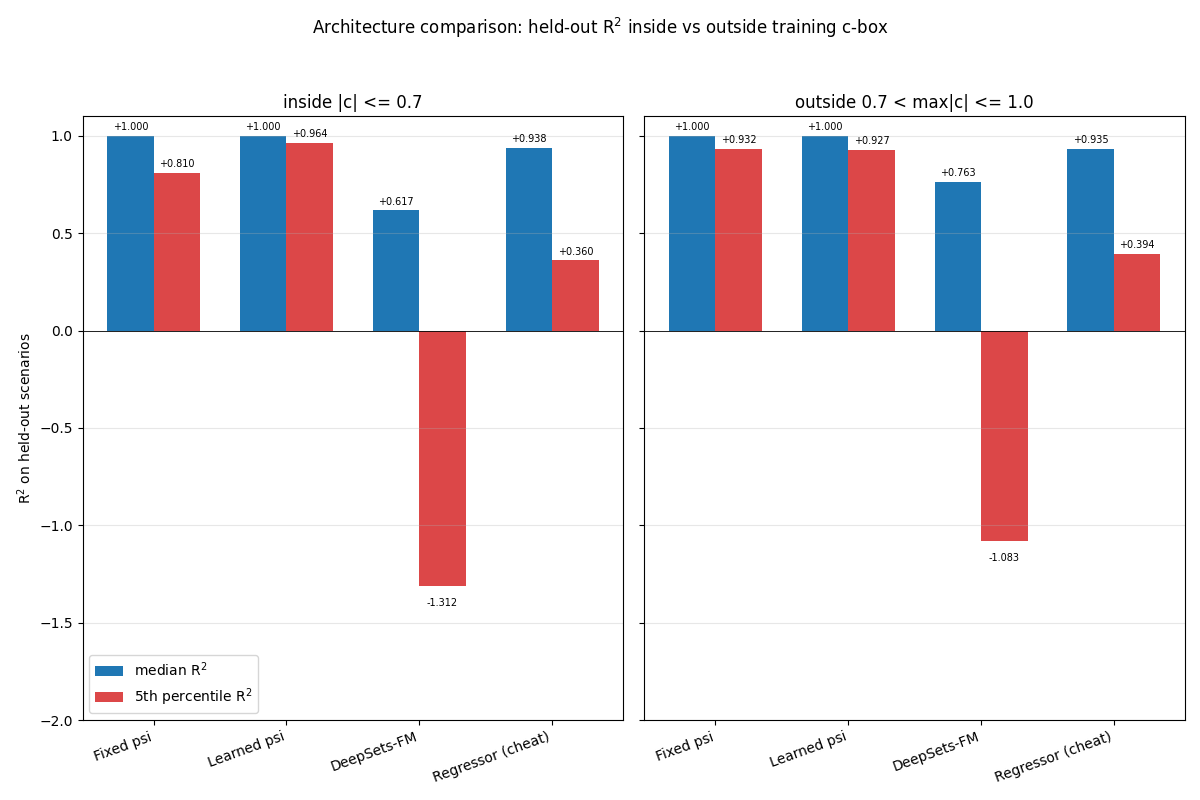
\includegraphics[width=0.85\linewidth]{figures/intention_vs_deepsets_inside_outside.png}
\caption{\label{fig:inside-outside} Median (solid) and fifth-percentile (hatched) coefficient of determination $R^2$ for the four architectures on the in-distribution ($|\bm{c}| \leq 0.5$, left) and out-of-distribution ($|\bm{c}| \in [0.5, 1.0]$, right) held-out scenarios. The Intention head with learned basis ($\psib_\theta$) reaches the highest fifth-percentile $R^2$ in both regions and beats the cheat regressor that violates the architectural constraint.}
\end{figure}

Figure~\ref{fig:curves} shows the predicted cross-section ratios alongside the ground truth on three representative held-out scenarios, chosen to span Standard-Model-like, energy-growing and interference-dominated regimes. The two Intention variants sit on top of the ground truth at every query point in all three scenarios. The DeepSets baseline follows the qualitative slope but biases high on rate-dominated scenarios and undershoots at low $\mll$. The cheat regressor produces small wobbles around the truth, consistent with a generic multilayer perceptron interpolating across the joint $(\bm{c}, \mll)$ space without an inductive bias for the closed-form polynomial structure. The qualitative picture matches the median and worst-case numbers in Table~\ref{tab:headline}.

\begin{figure}[t]
\centering
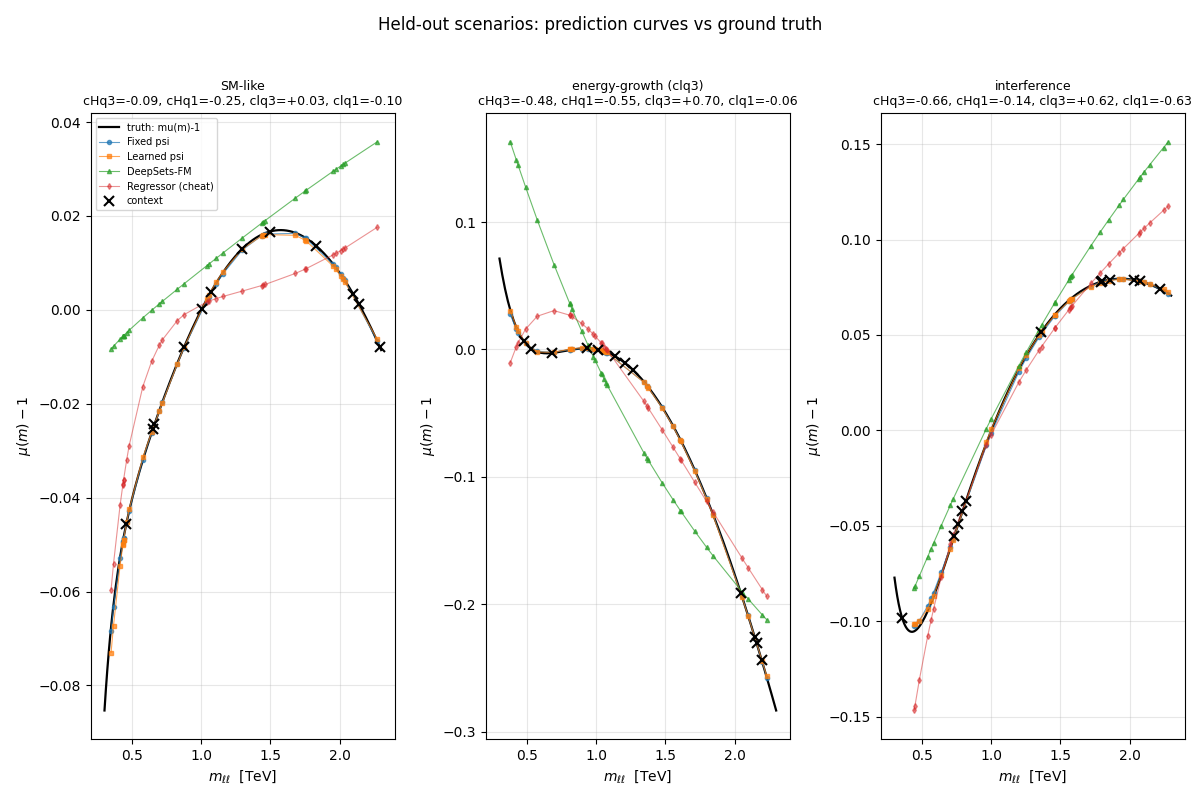
\includegraphics[width=\linewidth]{figures/intention_vs_deepsets_curves.png}
\caption{\label{fig:curves} Predicted cross-section ratio $Y(\mll) = \sigma(\bm{c}, \mll) / \sigsm(\mll)$ for three representative held-out scenarios: a Standard-Model-like configuration (left), an energy-growing configuration dominated by the four-fermion operators (centre) and an interference-dominated configuration (right). The two Intention variants trace the ground truth at every query point; the DeepSets baseline follows the slope but is biased; the cheat regressor produces small wobbles around the truth.}
\end{figure}

\subsection{Sample efficiency}

Figure~\ref{fig:scaling} reports the held-out median $R^2$ as a function of the number of Adam steps. The learned-basis Intention head reaches $R^2 > 0.96$ after a single optimiser step on $24$ scenarios, climbs to $R^2 > 0.98$ by step $25$, and saturates at $R^2 = 0.9997$ around step $1\,500$. The DeepSets baseline sits at $R^2 \ll 0$ for the first $\sim 50$ steps, crosses zero around step $600$, and reaches $0.617$ only by step $1\,500$. The two curves do not occupy the same regime of optimisation difficulty. The interpretation is that the closed-form attention machinery does almost all the inference work; the multilayer perceptron only needs to nudge $\psib_\theta$ into a basis in which the per-scenario ridge problem is well posed. Once that is achieved, the test error collapses to the ridge bias.

\begin{figure}[t]
\centering
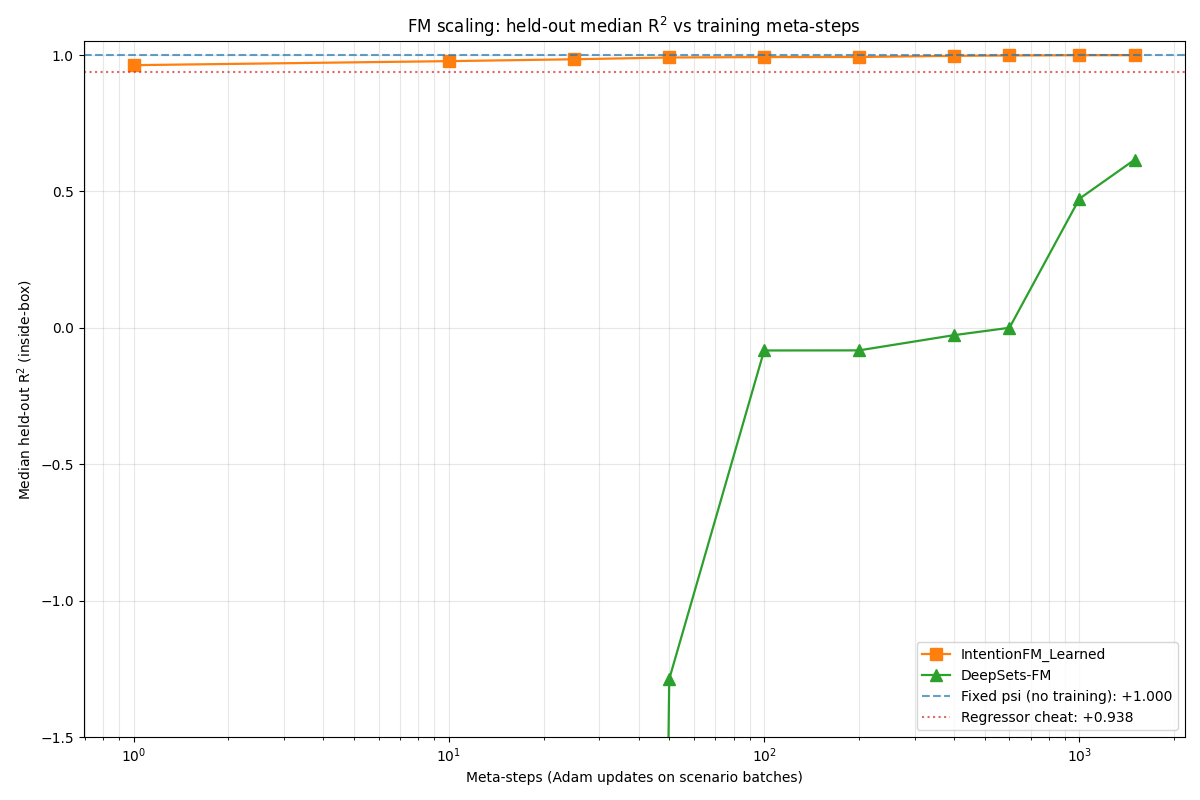
\includegraphics[width=0.85\linewidth]{figures/intention_vs_deepsets_scaling.png}
\caption{\label{fig:scaling} Held-out median $R^2$ on the in-distribution scenarios as a function of the number of meta-training steps, logarithmic in the abscissa. The learned-basis Intention head reaches $R^2 > 0.96$ after one optimiser step and saturates near $R^2 = 0.9997$ by step $1\,500$. The DeepSets baseline crosses $R^2 = 0$ near step $600$ and plateaus at $R^2 = 0.62$.}
\end{figure}

\subsection{The learned representation}

A natural question is whether the learned basis $\psib_\theta$ is, on this problem, simply a rediscovery of the polynomial basis used in the fixed variant. It is not. Figure~\ref{fig:psi-basis} shows the $16$ columns of $\psib_\theta$ alongside the $5$ columns of the fixed polynomial basis. The learned columns include features with localised bumps near $\mll \approx 0.4$~TeV and $\mll \approx 1.5$~TeV, sigmoid-like transitions in $\log m$, and tail-emphasising shapes that the fixed basis cannot represent. Several columns are visibly non-monotone. The fixed basis, by contrast, consists of $1, \log(m / \Mref), \ldots, \log^4(m / \Mref)$, that is, increasing polynomials in $\log m$.

\begin{figure}[t]
\centering
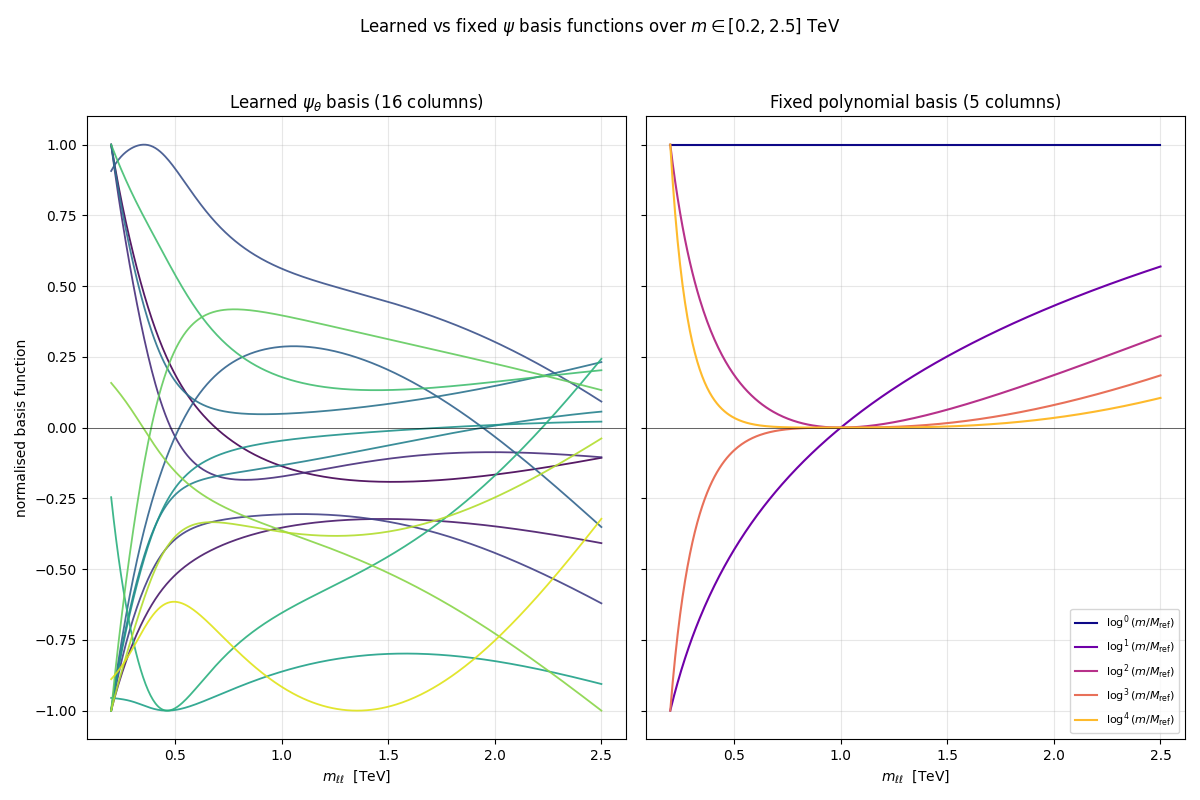
\includegraphics[width=\linewidth]{figures/intention_psi_basis.png}
\caption{\label{fig:psi-basis} The learned feature map $\psib_\theta : \mathbb{R} \to \mathbb{R}^{16}$ evaluated on a dense grid in $\mll$ (left, $16$ columns) and the fixed polynomial feature map $\psib(m) = \{1, \log(m/\Mref), \ldots, \log^4(m/\Mref)\}$ (right, $5$ columns). The learned columns include localised bumps near $\mll \approx 0.4$~TeV and $\mll \approx 1.5$~TeV and tail-emphasising shapes that the fixed basis cannot represent.}
\end{figure}

The difference is consistent with the small but significant gap in fifth-percentile $R^2$ between the two Intention variants in Table~\ref{tab:headline} ($0.964$ versus $0.810$ inside the training box). The fixed basis is sufficient for the median scenario, where the cross-section ratio is dominated by the leading polynomial behaviour, but it is brittle on tail scenarios in which the worst-conditioned polynomial columns blow up. The learned basis produces a more numerically stable ridge problem on those scenarios, at no cost to the median. We read this as the operational meaning of the foundation-model claim on this problem: the learned representation absorbs structure from the data manifold that the hand-engineered basis cannot encode.

\section{The full inference loop}
\label{sec:loop}

The closed-form attention head admits exact sequential updates by the Sherman-Morrison identity~\cite{Sherman:1950}: a new context observation $(\psib_\theta(M_{K+1}), Y_{K+1})$ updates the inverse design matrix $\bm{A}^{-1}$ in $\mathcal{O}(D^2)$ floating-point operations, with no gradient-descent step. This makes the model a natural primitive for a closed-loop inference system in which a foundation model encoder, a drift monitor, an active-learning acquisition function and a calibrator co-operate without retraining the underlying weights. We exhibit such a loop here, on an engineered out-of-distribution event designed to exercise every contract.

\subsection{Architecture}

The loop has four layers. The simulator, here the analytic oracle of Section~\ref{sec:theory}, supplies cross-section labels at chosen $(\bm{c}, \mll)$ on demand. The foundation model, the learned-basis Intention head of Section~\ref{sec:architecture}, supplies predictions and predictive variances at chosen query points. Three drift detectors monitor the residual stream and the design matrix. The acquisition function, the Expected Predictive Information Gain~\cite{Smith:2023epig} in its closed form under Bayesian linear regression (Appendix~\ref{app:derivations}), selects the next batch of kinematic points to query when drift fires. A leverage-stratified split-conformal calibrator~\cite{Lei:2018conformal,Vovk:2005alg} maintains finite-sample coverage on the predictive intervals.

The three drift detectors target distinct failure modes. Accuracy drift uses the Data-Adaptive Symmetric CUSUM~\cite{Ahad:2022dascusum} on standardised residuals $(Y_{\rm oracle} - \hat{Y}) / \hat{\sigma}$, with a sequential-change-point detector whose expected run length to false alarm is calibrated to $\sim 10^3$. Calibration drift uses the per-region binomial test on conformal interval coverage, with the Benjamini-Hochberg~\cite{Benjamini:1995fdr} correction across regions; we follow the recent treatment of Araz and Spannowsky~\cite{Araz:2025conformal} in adopting conformal prediction as the calibration substrate. Coverage drift uses the condition number $\kappa(\bm{A})$ of the design matrix; under the Eckart-Young theorem, $\kappa(\bm{A})$ upper-bounds the variance-amplification factor of the predictive variance along the worst-conditioned direction of feature space. An aggregator combines the three signals through a small decision table that chooses among recalibration, local retraining and global retraining, with persistence and cool-down rules that we describe in Appendix~\ref{app:derivations}.

The closed-form Information Gain admits a particularly simple expression in the Bayesian linear regression~\cite{Smith:2023epig}:
\begin{equation}
  \mathrm{IG}_T(p) \;=\; \frac{1}{2}\,\log\!\left(\frac{\mathrm{lev}_T}{\mathrm{lev}_T - k_{Tp}^2 / (\mathrm{lev}_p + 1)}\right),
  \quad k_{Tp} \;\equiv\; \psib_\theta(T)^\top \bm{A}^{-1} \psib_\theta(p),
  \label{eq:epig}
\end{equation}
with $T$ a target query and $p$ a candidate pool point. The Cauchy-Schwarz inequality on the $\bm{A}^{-1}$ inner product gives $k_{Tp}^2 \leq \mathrm{lev}_T \cdot \mathrm{lev}_p$, so the argument of the logarithm sits in $(0, 1]$ and the information gain is non-negative. The noise variance $\sigma_y^2$ cancels exactly under the homoscedastic assumption. We use a sequential-greedy implementation that updates $\bm{A}^{-1}$ by Sherman-Morrison after each selected point, which gives $\mathcal{O}(D^2)$ cost per acquisition.

The closed-form Bayesian linear regression also supplies a natural progress monitor for the loop, namely the target-set predictive entropy
\begin{equation}
  H_T \;=\; \frac{1}{2}\,\sum_{i=1}^{N_T}\,\log\!\bigl(2\pi e\, \sigma_y^2\, \mathrm{lev}_{T_i}\bigr),
  \label{eq:ht}
\end{equation}
which falls monotonically as the context grows and the leverage at each target shrinks. We use $H_T$ as the headline span attribute on every context-update event.

\subsection{The engineered drift event}

We pretrain the learned-basis Intention head on the analytic oracle with the band $|c_{\ell q}^{(3)}| \in [0.6, 1.0]$ excluded from the meta-training distribution, $1\,500$ Adam steps with the configuration of Section~\ref{sec:training}. The model is then queried at inference time in the withheld band, with target Wilson configuration $\bm{c} = (0, 0, 0.8, 0)$, from a thin seed context of $K = 8$ observations clustered in $\mll \in [0.5, 1.0]$~TeV. The four-fermion operator $\mathcal{O}_{\ell q}^{(3)}$ drives the cross-section ratio to a steeply energy-growing tail; under the $(\mll / \Lam)^4$ scaling at $\Lam = 1$~TeV, the ratio reaches $\mu(\mll) \approx 870$ at $\mll = 2.25$~TeV.

The closed-loop trial runs for $400$ cycles. Each cycle generates $24$ probe points (with $50\%$ tail-biased to $\mll > 1.5$~TeV), the model emits a prediction with conformal interval, the three drift detectors evaluate the residual stream, the aggregator selects an action, and if the action is local retraining the EPIG acquisition selects $k = 5$ kinematic points inside the drifted region, the oracle returns labels, the Intention context grows by five and the conformal calibrator is refit. The total oracle budget is $500$ calls, exhausted at cycle $\sim 300$; the remaining $100$ cycles continue running the model without acquisition.

\subsection{Recovery from the engineered drift}

Figure~\ref{fig:before-after} shows the foundation model prediction in the withheld band before and after the closed-loop run. Both panels use identical $\psib_\theta$ weights; only the context differs. The left panel, with the seed context of $K = 8$ observations clustered in $\mll \in [0.5, 1.0]$~TeV, shows the model's extrapolation flatlining at $\mu \approx 60$, root-mean-square error $293$ against the ground truth. The right panel, after $500$ oracle invocations across $100$ EPIG-driven acquisition events, shows the closed-form ridge solve on the grown context tracing the ground-truth curve at root-mean-square error $2.65$. The factor $110\times$ recovery is delivered with zero gradient-descent steps at inference. The model weights are unchanged from pretraining; the only state that has grown is the context.

\begin{figure}[t]
\centering

\includegraphics[width=\linewidth]{figures/chain_before_after.png}
\caption{\label{fig:before-after} Foundation model prediction in the withheld $|c_{\ell q}^{(3)}| \in [0.6, 1.0]$ band, target $\bm{c} = (0, 0, 0.8, 0)$. Both panels use identical $\psib_\theta$ weights. Left: thin seed context of $K = 8$ observations in $\mll \in [0.5, 1.0]$~TeV; the extrapolation flatlines at $\mu \approx 60$, root-mean-square error $293$. Right: after $500$ EPIG-driven oracle invocations across $100$ acquisition events, the context has grown to $508$ observations and the closed-form ridge solve traces the ground-truth curve at root-mean-square error $2.65$.}
\end{figure}

Figure~\ref{fig:trajectory} reports the four monitoring quantities through the run. The target-set predictive entropy $H_T$ of equation~(\ref{eq:ht}) falls monotonically from $+40$ to $-50$ over the $400$ cycles. The design-matrix condition number $\kappa(\bm{A})$ climbs from $10^3$ at seed context to $3 \times 10^5$ at full context; this is the signature of new directions being added to the basis row space as the context fills the withheld region, not a failure mode. The per-region empirical $68\%$ coverage stabilises into the $[0.65, 0.72]$ band within $\sim 40$ cycles and stays there once the loop reaches steady state. The oracle calls and context size grow linearly until the budget is exhausted.

\begin{figure}[t]
\centering

\includegraphics[width=\linewidth]{figures/chain_trajectory.png}
\caption{\label{fig:trajectory} Trajectories of the four monitoring quantities through the $400$-cycle closed-loop run. Top left: target-set predictive entropy $H_T$ from equation~(\ref{eq:ht}). Top right: design-matrix condition number $\kappa(\bm{A})$. Bottom left: per-region empirical $68\%$ coverage relative to the nominal target (dashed line). Bottom right: cumulative oracle calls (green) and context size (orange).}
\end{figure}

Figure~\ref{fig:drift-events} reports the drift detectors firing in real time and the aggregator actions. The Data-Adaptive Symmetric CUSUM fires episodically whenever the residual stream's standardised median departs from zero. The per-region binomial $p$-value, in logarithmic scale, plunges below the nominal $\alpha = 0.05$ whenever any of the five $\mll$-regions under- or over-covers. The aggregator stripe shows local-retraining firings dominating the first $\sim 300$ cycles, with budget-exhausted cycles dominating the remaining $100$, during which the recovered prediction holds.

\begin{figure}[t]
\centering
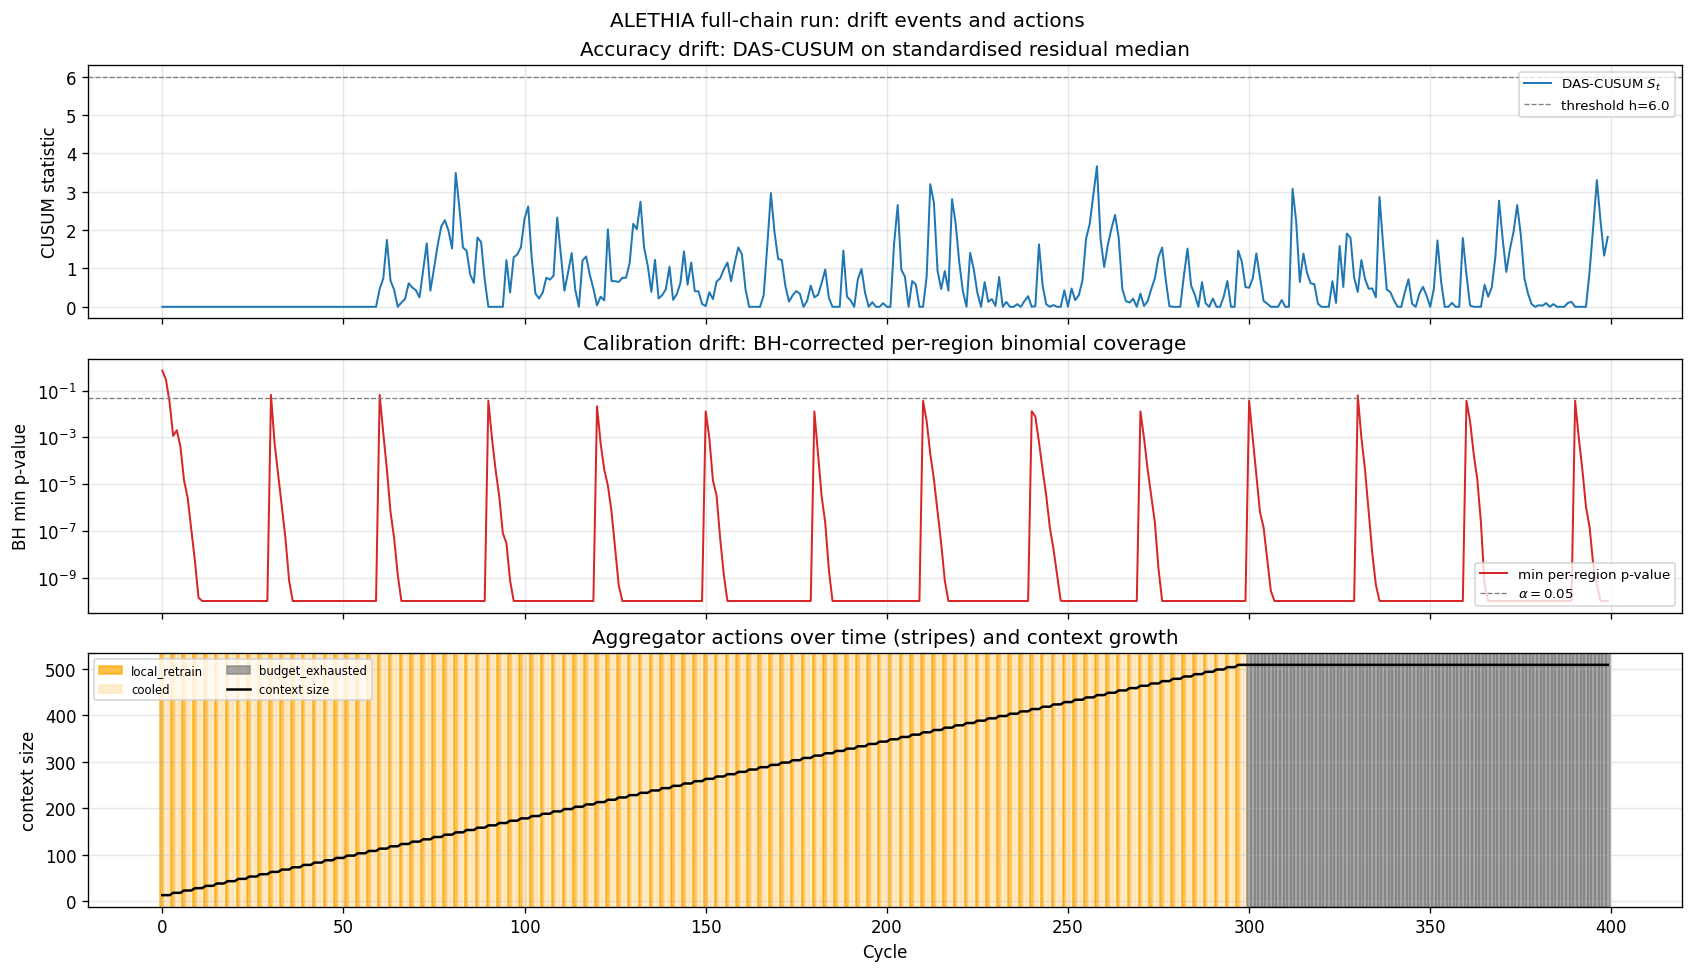
\includegraphics[width=\linewidth]{figures/chain_drift_events.png}
\caption{\label{fig:drift-events} Drift detectors and aggregator actions through the closed-loop run. Top: Data-Adaptive Symmetric CUSUM on the standardised residual median. Middle: per-region minimum $p$-value of the binomial coverage test with the Benjamini-Hochberg correction across the five regions, on a logarithmic vertical axis. Bottom: aggregator action per cycle (orange stripes for local retraining, grey for budget-exhausted) with context size overlaid.}
\end{figure}

The root-mean-square error trajectory in Fig.~\ref{fig:rmse-recovery} confirms that the loop spends its entire runtime in the $[2.4, 2.95]$ band on the target region, distinct from the standalone seed-context root-mean-square error of $293$. The early growth between cycles $0$ and $\sim 8$ is the model accommodating the first round of EPIG-supplied tail observations, which transiently perturb the ridge solve; from cycle $\sim 30$ onward the root-mean-square error settles at $\approx 2.65$.

\begin{figure}[t]
\centering

\includegraphics[width=0.85\linewidth]{figures/chain_rmse_recovery.png}
\caption{\label{fig:rmse-recovery} Root-mean-square error of the foundation model on the $50$-point target band over the $400$ cycles, on a logarithmic vertical axis. Vertical orange marks indicate EPIG-driven acquisition events (one hundred in total). The standalone seed-context root-mean-square error of $293$ is not visible at this scale.}
\end{figure}

\section{Discussion}
\label{sec:discussion}

The headline benchmark of Section~\ref{sec:results} uses the polynomial-toy oracle of Section~\ref{sec:training}, whose closed form is a quartic polynomial in $\log(\mll / \Mref)$ at fixed Wilson coefficients. The fixed-basis Intention variant has the exact analytic structure of the target function written into its feature map, and its near-perfect median $R^2$ is therefore a tautology rather than evidence in favour of the fixed basis on the full Drell-Yan calculation. The learned-basis variant is not exploiting this; the basis it discovers is not a rediscovery of the polynomial and the fifth-percentile $R^2$ gap between the two variants ($0.964$ versus $0.810$ in-distribution) is consistent with the learned basis solving the per-scenario ridge problem more stably on tail scenarios. We expect, but do not yet demonstrate, that on the full next-to-next-to-leading-order calculation with parton distribution function thresholds and resonance structure the gap between the learned and fixed bases will grow.

The DeepSets baseline is at an architectural disadvantage on a one-dimensional kinematic regression problem. The mean-pool encoder summarises the context through a fixed-dimensional vector that aggregates the per-event embeddings, which discards the alignment between $M_{{\rm ctx}, i}$ and $Y_{{\rm ctx}, i}$ that the closed-form ridge solve exploits. The decoder then has to invert, by gradient descent over training scenarios, a hashed summary of the context, which is a substantially harder problem than solving a $16 \times 16$ linear system. The fact that DeepSets performs better outside the training $\bm{c}$-box than inside it (median $R^2 = 0.76$ versus $0.62$) is a giveaway: the inside-box scenarios have small excursions of $Y(\mll)$ around the Standard-Model curve where the mean pool cannot resolve them, while the outside-box scenarios have larger excursions where any reasonable encoder can latch onto the dominant direction.

Extending the Intention head from a one-dimensional kinematic variable to multi-dimensional event-level kinematics is the natural next step. The closed-form attention applies most cleanly when the input to each context entry is a fixed-length feature vector; on event sets one can either pool to a fixed-length representation, which re-introduces the DeepSets failure mode, or treat each event as its own context entry, which makes $K$ equal to the number of events and the linear-system cost grow with the third power of the basis dimension. The most plausible hybrid, which we leave for future work, uses a Particle Transformer~\cite{Qu:2022part} or DeepSets event encoder to produce a fixed-length representation of the context, which is then fed as the $\psib_\theta$ rows of the Intention head. We conjecture that the architecture survives this hybridisation, on the grounds that the closed-form ridge solve is feature-map-agnostic.

The closest physics-side antecedents of the present work are the parametrised-classifier line of Chen, Glioti, Marzocca, Nardini and Wulzer~\cite{Chen:2022lcp} and the joint-likelihood-ratio line of Brehmer, Cranmer, Louppe and Pavez~\cite{Brehmer:2018kdj}. Both lines fit a network per Wilson configuration sampled at training time, and re-evaluate the fit at deployment by interpolating across the trained Wilson grid. The present model amortises the inference rather than the conditional density: a single learned feature map handles arbitrary Wilson configurations through the context, with the only inference-time cost a matrix solve in a sixteen-dimensional space. The price is that the model is restricted to the observable representation in which $\psib_\theta$ is defined, which here is binned cross-section ratios. The closest in-context antecedent is the Prior-Fitted Network construction~\cite{Mueller:2022pfn}, where a transformer is pretrained on synthetic datasets sampled from a prior such that a single forward pass with a context set produces an approximate Bayesian posterior predictive. Our model adopts the same in-context view, but with the closed-form linear attention of equation~(\ref{eq:intention}) in place of the generic transformer.

The jet-level foundation model literature~\cite{Mikuni:2024omnilearn,Mikuni:2025omnilearned,Heinrich:2024mpm,Birk:2024omnijet,Katel:2025hepjepa,Sophon:2024} addresses a distinct task family. Those models are trained on large simulated jet corpora and evaluated on jet classification benchmarks, with success measured by area under the receiver-operating-characteristic curve and background rejection at fixed signal efficiency. The closest analogue of our setting in that cluster is the OmniLearn fine-tuning evaluation~\cite{Mikuni:2024omnilearn,Mikuni:2025omnilearned}, which reports sample-efficiency benefits on classification when the pretrained backbone is fine-tuned on small downstream labelled sets. We do not attempt a comparison to those benchmarks, because our model produces a continuous prediction of a cross-section ratio rather than a class probability; the underlying inference problem is different.

A persistent silence in the jet-level foundation model literature is uncertainty quantification on the model's outputs. Calibration curves, conformal coverage and posterior-predictive checks are rarely reported. The present work adopts conformal prediction as the calibration substrate, following the recent treatment of Araz and Spannowsky~\cite{Araz:2025conformal}, and reports per-region empirical coverage as a primary diagnostic of the closed-loop run. We regard this as a complementary contribution: the active-learning loop of Section~\ref{sec:loop} is gated by calibration drift, and a foundation model without honest predictive intervals cannot supply the trigger.

\section{Summary and outlook}
\label{sec:conclusions}

We have presented a closed-form attention foundation model for amortised inference of dimension-six SMEFT effects in Drell-Yan. The model is trained end-to-end through a closed-form ridge inversion in a learned feature map, with the architectural constraint that the Wilson coefficient never enters the forward pass. On a controlled benchmark over fifty in-distribution and fifty out-of-distribution Wilson configurations the model reaches median $R^2 = 0.9997$ and fifth-percentile $R^2 = 0.93$, against $0.62$ and $-1.08$ respectively for a parameter-matched DeepSets baseline, and beats a regressor that violates the constraint and receives the Wilson vector for free at test time. The learned basis is visibly not a rediscovery of the canonical polynomial features. The model composes into a closed-loop inference system in which physics-aware drift detectors gate an EPIG-driven acquisition step and a conformal calibrator maintains coverage; on an engineered out-of-distribution event the loop recovers from a root-mean-square error of $293$ to $2.65$ in $500$ oracle calls with no gradient-descent step at inference.

The most immediate extension is from the one-dimensional binned-distribution observable used here to multi-dimensional event-level kinematics. We expect the closed-form ridge solve to survive a hybridisation in which a Particle Transformer or DeepSets event encoder produces the rows of the Intention head, on the grounds that the inference-time solve is feature-map-agnostic; the integration is left for future work. Replacing the analytic leading-order oracle with a next-to-next-to-leading-order calculation that exposes parton distribution function thresholds and realistic detector smearing is similarly within reach: the closed-loop monitoring infrastructure carries over without modification, and the fixed-basis variant is expected to lose ground to the learned basis on the threshold structure. The propagation of the closed-loop output through to published confidence intervals on individual Wilson coefficients, with the conformal coverage providing the calibration guarantee, is the cleanest physics deliverable that the present infrastructure enables, and is the form in which we will report the next iteration of this work. A systematic study of the in-context generalisation behaviour as a function of the size and diversity of the meta-training scenario distribution, following the scaling-behaviour analyses now standard in the jet-level foundation model literature, is a parallel direction that would establish whether the closed-form attention head exhibits the same power-law scaling reported for transformer-based foundation models on jet corpora.

\section*{Acknowledgements}

The agent runtime is built on the Google Agent Development Kit and the trace pipeline is built on Arize Phoenix; this work is the author's entry to the Arize track of the Google Cloud Rapid Agent Hackathon. The closed-form attention pattern is from Garnelo and Czarnecki~\cite{Garnelo:2023intention}. The conformal-prediction substrate follows Araz and Spannowsky~\cite{Araz:2025conformal}. The SMEFT cross-section calculator is built directly from the dimension-six amplitude decomposition in Greljo and Marzocca~\cite{Greljo:2017vvb}, with Warsaw-basis operators following Grzadkowski, Iskrzynski, Misiak and Rosiek~\cite{Grzadkowski:2010es}.

\appendix

\section{Closed-form derivations}
\label{app:derivations}

\subsection{Sherman-Morrison sequential update}

Given the inverse design matrix $\Ainv$ at context size $K$ and a new context entry with feature vector $\psib_p = \psib_\theta(M_{K+1})$, the Sherman-Morrison identity~\cite{Sherman:1950} gives the rank-one update
\begin{equation}
  \bm{A}_{\rm new}^{-1} \;=\; \Ainv \;-\; \frac{(\Ainv \psib_p)(\psib_p^\top \Ainv)}{1 + \psib_p^\top \Ainv \psib_p},
  \label{eq:sm}
\end{equation}
which is exact to numerical precision. Equation~(\ref{eq:sm}) costs $\mathcal{O}(D^2)$ floating-point operations and admits a streaming implementation; the foundation model context can grow by one observation per Sherman-Morrison invocation, with the inverse design matrix maintained as a cache.

\subsection{Closed-form Information Gain}

The Expected Predictive Information Gain~\cite{Smith:2023epig} on a target distribution $T$ from the addition of a candidate pool point $p$ is, in the Bayesian linear regression on the basis $\psib_\theta$,
\begin{equation}
  \mathrm{IG}_T(p) \;=\; \mathbb{E}_{T}\!\left[\,\frac{1}{2}\,\log\!\left(\frac{\sigma_T^2}{\sigma_{T \mid p}^2}\right)\right]
  \;=\; \frac{1}{2}\,\log\!\left(\frac{\mathrm{lev}_T}{\mathrm{lev}_T - k_{Tp}^2 / (\mathrm{lev}_p + 1)}\right),
\end{equation}
where the second equality uses equation~(\ref{eq:sm}) to express the post-update leverage $\mathrm{lev}_{T \mid p}$ in terms of pre-update quantities. The Cauchy-Schwarz inequality on the $\Ainv$ inner product gives $k_{Tp}^2 \leq \mathrm{lev}_T \cdot \mathrm{lev}_p$, so the argument of the logarithm sits in $(0, 1]$ and the information gain is non-negative. The noise variance $\sigma_y^2$ cancels exactly under the homoscedastic assumption used in the ridge fit.

\subsection{Aggregator decision rules}

The drift aggregator combines the three detector outputs through an eight-row table indexed by the binary states of accuracy, calibration and coverage drift. When only coverage drift fires, the action is local retraining inside the drifted region. When only calibration drift fires, the action is recalibration of the conformal calibrator. When all three fire, the action is global retraining. The aggregator implements two persistence rules. A calibration-only fire that recurs for four consecutive cycles escalates to local retraining. An accuracy-only fire requires three consecutive cycles before triggering oracle calls. A cool-down of three cycles between consecutive local-retraining firings prevents the loop from issuing back-to-back acquisition calls on the same drift event.

\section{Reproduction}
\label{app:reproduction}

All experiments reported in this paper run on a single central-processing-unit. The closed-form attention head and the meta-learning objective are implemented in PyTorch via the differentiable solver \texttt{torch.linalg.solve}. The analytic oracle is implemented in NumPy with parton distribution functions supplied by LHAPDF~\cite{Buckley:2014lhapdf} using the CT18NNLO set~\cite{Hou:2019ct18}. The closed-loop run, including drift detection, EPIG acquisition and conformal recalibration, completes in $\sim 17$ minutes of pretraining and a further $19$ seconds of loop time. Phoenix is run locally in a Docker container and ingests OpenTelemetry spans through OpenInference instrumentation; the rubric MCP queries against the resulting trace tree are answered as single-span filters. The full source for the experiments and the closed-loop run is in the project repository at \texttt{experiments/intention-vs-deepsets/} and \texttt{experiments/full-chain-run/}.

\bibliographystyle{unsrtnat}
\bibliography{alethia}

\end{document}
